\documentclass[conference]{IEEEtran}
\usepackage{cite}
\usepackage{amsmath,amssymb,amsfonts}
\usepackage{graphicx}
\usepackage{textcomp}
\usepackage{xcolor}
\usepackage{url}
\usepackage{tikz}
\usetikzlibrary{shapes.geometric, arrows.meta, positioning}
\usepackage[hidelinks,breaklinks]{hyperref}
\def\BibTeX{{\rm B\kern-.05em{\sc i\kern-.025em b}\kern-.08em
    T\kern-.1667em\lower.7ex\hbox{E}\kern-.125emX}}
\begin{document}

\title{The RAMNET Protocol: A Decentralized Universal Compute Mesh for Heterogeneous Hardware}

\author{\IEEEauthorblockN{Kevin West}
\IEEEauthorblockA{\textit{RAMNET Project} \\
westkevin12@github.com}}

\maketitle

\begin{abstract}
The RAMNET Protocol addresses the ``Thermodynamic Wall'' of centralized AI by introducing a heterogeneous, decentralized compute mesh. By leveraging NVIDIA Rubin-class digital GPUs for training, Mythic analog processors for edge inference, and IBM quantum-ready logical qubits, RAMNET constructs a contiguous virtual address space. We propose a high-performance Layer 3 (L3) execution environment for state persistence, utilizing a 6-node ECC (Error Correction Code) redundancy model. This separates ``Ephemeral Compute Traffic'' from ``L1 Consensus Logic,'' ensuring ultra-low shard coordination latency for autonomous agent coordination while maintaining public immutability for verification.
\end{abstract}

\begin{IEEEkeywords}
Distributed Shared Memory (DSM), Analog Compute, 6-Node ECC, Layer 3 Persistence, Post-Quantum Security.
\end{IEEEkeywords}

\section{Introduction: The Next Evolutionary Pivot}
The history of artificial intelligence is defined by hardware-driven breakthroughs. The shift from general-purpose CPUs to massively parallel GPUs unlocked the Era of Transformers by solving the memory and algorithmic bottlenecks of early neural networks. Today, centralized compute has reached its thermodynamic limit. A single NVIDIA H100 SXM GPU draws 700 Watts, and global AI data center capacity demand is projected to rise 33\% annually through 2030 \cite{mckinsey2024ai}. Centralized clusters waste 80--90\% of peak capacity on idle time and cooling, while edge devices sit underutilized. RAMNET turns every idle GPU, Mythic analog tile, and future quantum module into a seamless, pay-per-shard global RAM fabric\footnote{PulseChain selected for initial L1 coordination due to high throughput and ultra-low transaction fees; multi-chain bridges to Ethereum and Solana are planned for later phases.}.

The RAMNET Protocol represents the next evolutionary pivot. To unlock the next frontier of performance driven by the scaling of \textbf{Larger Models + More Data + More Hardware} the industry must transition to heterogeneous, energy-efficient analog mesh compute. Analog compute is the necessary pivot for edge inference. The Mythic M1076 Analog Matrix Processor delivers 25 TOPS at an $\approx$3W power envelope, achieving 100x better energy efficiency than digital GPUs \cite{mythic2024m1076}.

\subsection{Operational Overview}
The RAMNET workflow streamlines complex orchestration into a cohesive pipeline:
\begin{enumerate}
    \item \textbf{Submission:} A user submits a large model training or inference task.
    \item \textbf{Decomposition:} A Gateway Node decomposes the task into ``blind'' matrix logic hashes.
    \item \textbf{Sharding:} Apache Spark orchestrates the splitting of logic into a 3-way dimensional matrix split (row, column, and reduction slices) across 6-node groups.
    \item \textbf{Execution:} Digital nodes (NVIDIA Rubin) handle pre-training, while analog nodes (Mythic) run efficient inference passes.
    \item \textbf{Verification:} Results are recombined via Verde-style bisection, with Tier-4 nodes resolving rare disputes.
    \item \textbf{Settlement:} Rewards flow via SCU-normalized PoUW on the PulseChain coordination layer.
\end{enumerate}

\section{Hardware Orchestration \& NVIDIA Integration}
To achieve the ultra-low coordination latency required for RAMNET, we integrate NVIDIA's 2026 Rubin Architecture \cite{nvidia2026rubin}. Unlike legacy systems, Rubin utilizes HBM4 (High Bandwidth Memory) and the NVLink-6 Switch System, providing up to 3,600 GB/s of GPU-to-GPU throughput and rack-scale aggregate bandwidth of 260 TB/s. RAMNET abstracts these digital powerhouses alongside Analog Matrix Processors and quantum-ready logical qubits, aligning with long-term industry roadmaps for logical qubit scaling \cite{ibm2024roadmap}. While NVIDIA handles the heavy ``Pre-training'' (Global Logic), the Analog nodes handle the ``Inference'' (Local Logic), reducing total mesh power consumption by an estimated 80\%.

\section{The Data Backplane: Spark \& Sharded Persistence}
We utilize Apache Spark as the orchestration engine for distributed data frames across the mesh. Spark's RDD (Resilient Distributed Dataset) logic is extended into the RAMNET DSM (Distributed Shared Memory), building upon established paradigms for transparent remote memory access \cite{wiki2024dsm}.

\subsection{L3 Sharded Persistence and Latency-Optimized Interconnect}
To avoid the ``Blockchain Bottleneck,'' we deploy an EVM-compatible L3 as a high-speed ``Cache Layer.'' This layer is critical for mitigating decentralized latency (10--200 ms) typically encountered across wide-area networks (WAN). By extending Apache Spark's RDD logic into a globally persistent L3 cache, RAMNET ensures that matrix operation states remain accessible to the mesh without requiring repetitive L1 state-root validation, achieving orchestration speeds orders-of-magnitude faster than L1 block times. \textbf{Challenges \& Roadmap:} Initial L3 implementation will leverage EVM-compatibility for developer accessibility, with future upgrade paths toward a Move-based VM for optimized matrix operation tracking.

\subsection{The 6-Node ECC "Global RAM" Model}
To mirror server-grade ECC RAM and hardware-level mirroring (e.g., redundant power supplies and RAID arrays), we implement a double-triplicate redundancy model. While the redundancy factor remains constant per compute task, the total mesh throughput scales linearly ($O(n)$) with the number of parallel nodes. This architecture ensures that the mesh functions as a self-healing memory space with no single point of failure.

\begin{figure}[htbp]
\centering
\resizebox{\columnwidth}{!}{
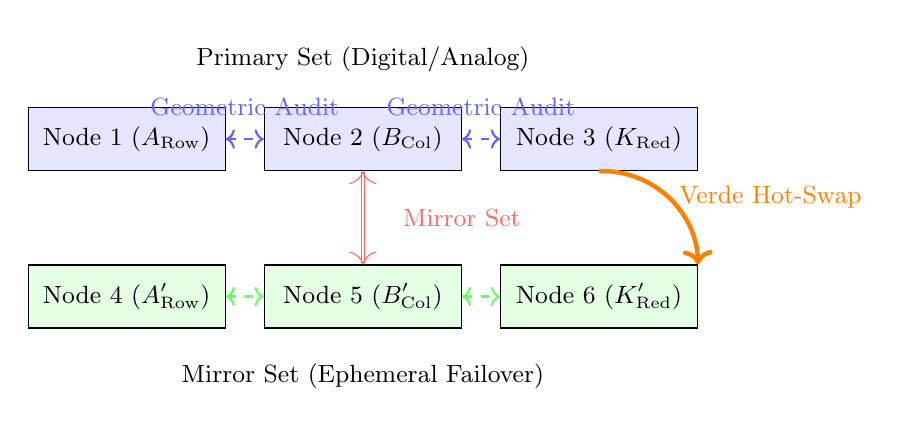
\begin{tikzpicture}[node distance=1.5cm, every node/.style={draw, rectangle, minimum width=2.5cm, minimum height=0.8cm, font=\small}]
    % Primary Set
    \node (n1) [fill=blue!10] {Node 1 ($A_{\text{Row}}$)};
    \node (n2) [right of=n1, xshift=1.5cm, fill=blue!10] {Node 2 ($B_{\text{Col}}$)};
    \node (n3) [right of=n2, xshift=1.5cm, fill=blue!10] {Node 3 ($K_{\text{Red}}$)};
    
    % Mirror Set
    \node (n4) [below of=n1, yshift=-0.5cm, fill=green!10] {Node 4 ($A'_{\text{Row}}$)};
    \node (n5) [below of=n2, yshift=-0.5cm, fill=green!10] {Node 5 ($B'_{\text{Col}}$)};
    \node (n6) [below of=n3, yshift=-0.5cm, fill=green!10] {Node 6 ($K'_{\text{Red}}$)};
    
    % Overlap Connectors (Audit Zones)
    \draw[<->, dashed, thick, blue!60] (n1.east) -- node[above, draw=none, fill=none] {Geometric Audit} (n2.west);
    \draw[<->, dashed, thick, blue!60] (n2.east) -- node[above, draw=none, fill=none] {Geometric Audit} (n3.west);
    
    % Mirror Set Connectors
    \draw[<->, dashed, thick, green!60] (n4.east) -- (n5.west);
    \draw[<->, dashed, thick, green!60] (n5.east) -- (n6.west);
    
    % Mirror Connection
    \draw[double, <->, red!60] (n2.south) -- node[right, draw=none, fill=none] {Mirror Set} (n5.north);
    
    % Hot-Swap Indicators
    \draw[->, ultra thick, orange, bend left=45] (n3.south) to node[right, draw=none, fill=none, orange] {Verde Hot-Swap} (n6.north east);
    
    % Group Labels
    \node[draw=none, above=0.2cm of n2] {Primary Set (Digital/Analog)};
    \node[draw=none, below=0.2cm of n5] {Mirror Set (Ephemeral Failover)};
\end{tikzpicture}
}
\caption{6-Node ECC Model: 3-Way Dimensional Matrix Decomposition with Natural Intersection Audit Zones and High-Durability Mirroring.}
\label{fig:ecc_model}
\end{figure}

\begin{itemize}
    \item \textbf{3-Way Dimensional Matrix Decomposition:} Tasks are partitioned across functional dimensions (row, column, and reduction axis slices). This achieves zero-overhead sharding while creating natural geometric audit intersections between adjacent nodes.
    \item \textbf{Mirror Set (Nodes 4-6):} A simultaneous, ephemeral duplicate of the dimensional split. This set acts as a fallback for surviving regional outages and global network partitions.
\end{itemize}
Totaling 6 nodes, if any single node fails or returns malicious data, the mesh uses the Verde Bisection Game to hot-swap the corrupted memory segment without dropping the compute task. This mechanism, adapted from Gensyn's referee-delegation model \cite{gensyn2025verde}, utilizes a two-level binary search on operations to pinpoint divergence at the logic-state level. Achieving ``Uninterruptible Compute,'' the protocol utilizes a competition-based incentive model where the first nodes to verify and return results receive the majority of the \$RAM reward, incentivizing the adoption of modern, high-performance hardware.

\subsection{Task Hardware Routing \& Fidelity}
RAMNET treats the global mesh as a unified system-on-chip (SoC). The runtime functions as a hardware-aware scheduler, routing high-precision training tasks to digital Rubin clusters and noise-tolerant inference shards to analog Mythic tiles. Because tasks are typed at the decomposition layer, \textbf{Precision Drift} is treated as a known environment parameter of the task context rather than a software regression. 

To maintain consensus across heterogeneous hardware, we implement \textbf{Range-Based Verification}. While digital results require bit-for-bit parity, analog results are validated against a statistically expected tolerance range ($\sigma$). The Verde Bisection Game is onlyEscalated to Tier 4 if an output falls outside this threshold, distinguishing natural hardware variance from malicious data corruption or work falsification.
\subsection{Interoperability and Abstraction Challenges}
Unifying digital GPUs, analog AI tiles, and quantum logical qubits requires a sophisticated abstraction layer. The RAMNET runtime acts as a universal compiler, decomposing high-level logic hashes ($\mathcal{H}_L$) into hardware-specific kernels. Analog devices receive primitive matrix-vector multiplication (MVM) operations where weights are pre-loaded, while dDigital devices (Rubin clusters) handle dynamic algorithmic branching, while quantum-ready nodes are reserved for specialized proof primitives or act as high-integrity oracles within the mesh. \textbf{Challenges \& Roadmap:} Heterogeneous execution requires a custom abstraction runtime (currently in development). Initial prototypes focus on digital-analog orchestration, with quantum-ready tiers phased in post-2027.

\section{Mathematical Proof: 6-Node Redundant ECC Model}
\subsection{3-Way Dimensional Matrix Decomposition}
Let a matrix multiplication task $T = A \times B$ with dimensions $M \times N$ and inner dimension $K$ be distributed across the mesh. Rather than dividing the total workload into overlapping linear segments which breaks cache locality, the task is partitioned across three distinct spatial dimensions:
\begin{equation}
\text{Shard}_A = A_{\left[0:\frac{M}{3}\right]} \times B \quad (\text{Row Projection})
\end{equation}
\begin{equation}
\text{Shard}_B = A \times B_{\left[0:\frac{N}{3}\right]} \quad (\text{Column Projection})
\end{equation}
\begin{equation}
\text{Shard}_C = A_{\left[:, 0:\frac{K}{3}\right]} \times B_{\left[0:\frac{K}{3}, :\right]} \quad (\text{Inner Reduction})
\end{equation}
The intersection where these dimensional calculations cross paths forms a natural, zero-overhead ``Audit Zone.'' Since these intersections are computed independently by distinct nodes, they act as unforgeable proof matrices to verify execution integrity without work duplication.

\subsection{Slashing and Sovereign Auditing}
Assuming the protocol requires a supermajority of at least 4 honest nodes to accept a shard result, the probability $P_{attack}$ of a corrupted or malicious result being accepted in a single task is:
\begin{equation}
P_{attack} \approx \sum_{k=4}^{6} \binom{6}{k} f^k (1-f)^{6-k}
\end{equation}
where $f$ is the fraction of malicious nodes in the global mesh and $k \geq 4$ is the threshold for overcoming the 6-node consensus. For a conservative mesh state where $f = 0.05$, the probability of an undetected malicious result is $P_{attack} < 1.0 \times 10^{-6}$, achieving server-grade reliability through statistical redundancy. Beyond malicious collision, nodes are subject to sovereign slashing for:
\begin{itemize}
    \item \textbf{High Latency:} Indications of poor-quality hardware or bandwidth limiting mesh throughput.
    \item \textbf{Privacy Violations ("Sniffing"):} Detection of unauthorized data traversal patterns during blind execution.
    \item \textbf{Work Falsification:} Submission of invalid computation hashes or faked proof-of-useful-work.
\end{itemize}
\subsection{Tiered Dispute Resolution}
In cases where an audit zone produces divergent results and a bisection game is contested, the protocol escalates the task to Tiered Dispute Resolution. Contested shards are re-executed by a Tier 4 (Quantum Ready) node. These nodes act as high-integrity oracles, running verifiable quantum-assisted computation or leveraging IBM's error-corrected logical qubits once utility-scale availability is reached. This provides a definitive cryptographic signature of the truth to resolve the dispute and execute slashing on the malicious auditor or provider. \textbf{Challenges \& Roadmap:} Quantum dispute resolution is a long-term milestone, contingent on the maturation of modular fault-tolerant quantum modules (targeted post-2028).

\section{Hyperscale Task Scaling and Durability}
The RAMNET protocol introduces a dynamic task scaling mechanism for ``Impossibly Large'' computations. While the 6-node ECC model provides a baseline for reliability, the protocol allows tasks to be partitioned across multiples of 3 nodes (e.g., 9, 12, 15), extending up to the entire mesh network. This allows for the execution of workloads that exceed the physical capacity of any single centralized cluster, enabling the training and inference of larger models with unprecedented data volumes. 

This scaling isn't merely for speed; it provides ``Extreme Durability,'' allowing computations to survive massive global network disruptions. Such hyperscale tasks are priced at a premium in \$RAM tokens to reflect the increased coordination overhead and resource lock-in across the mesh.

\section{The Resource Market and SCU Normalization}
The RAMNET economy functions as a high-frequency marketplace for heterogeneous compute. To ensure fair pricing across varied hardware tiers, the protocol utilizes the Standard Compute Unit (SCU). \textbf{Definition:} One SCU is defined as $10^{12}$ normalized floating-point or fixed-point matrix multiply-accumulate (MAC) operations, equivalent to a standardized FP16 GEMM kernel on NVIDIA Rubin-class hardware.
Nodes earn \$RAM based on their SCU throughput, hardware uptime, and verification accuracy. This allows an analog Mythic tile and an NVIDIA Rubin cluster to compete on the same market, with prices adjusting dynamically based on real-time mesh supply and demand.

Furthermore, we mitigate ``Cold-Start'' latency through \textbf{Warm Standby Rebates}. Nodes receive a baseline \$RAM performance multiplier for maintaining an active, compute-ready environment. Unlike passive participation, these rebates only unlock upon a successful task payout trigger. If a node fails to accept a routed task or misses an execution deadline (Liveness Slashing), the standby multiplier is forfeited, ensuring only nodes with genuine capacity and bandwidth capture mesh incentives.

Most modern hardware remains idle for a significant fraction of its lifecycle; the RAMNET protocol enables owners to monetize these idle cycles by providing them as an elastic resource to the mesh. While platforms like Akash \cite{akash2024}, Flux \cite{flux2024}, and Gensyn \cite{gensyn2024} have pioneered decentralized compute provisioning, RAMNET's edge lies in its universal hardware abstraction bridging digital, analog, and quantum resources into a single cohesive mesh. For compute consumers, this eliminates the waste of fixed-term cloud leases, replacing them with a fluid, bid-style marketplace where they pay only for the exact resources (CPU, GPU, Analog, Quantum, and RAM) consumed.

\section{Privacy Architecture: Logic-Data Decoupling}
To resolve the ``Privacy-Compute Paradox,'' RAMNET implements Logic-Data Decoupling. Tasks are functionally decomposed into abstract mathematical logic, stripping away raw data before distribution to the mesh. This ensures that nodes perform ``Blind Execution,'' where they process matrix operations without semantic context. Furthermore, data is protected by NIST-standard Post-Quantum algorithms, such as Crystals-Kyber, and leverages advancements in Fully Homomorphic Encryption (FHE) to maintain end-to-end sovereignty \cite{zama2024, nist2024pqc}. This architectural choice ensures that even a total mesh breach only reveals mathematically indigestible noise.

\section{Layered Settlement Architecture}
RAMNET strictly decouples Compute Work from Value Settlement:
\begin{itemize}
    \item \textbf{L1 (Ethereum / PulseChain / Solana):} Bridges, governance, and \$RAM token minting.
    \item \textbf{L2 (Arbitrum/Optimism):} General contract state and identity verification.
    \item \textbf{L3 (RAMNET Custom):} High-speed Cache Layer for the mesh.
\end{itemize}

\section{Gateway Nodes and Orchestration Throughput}
For users with low-compute local hardware (e.g., mobile devices or IoT sensors), the protocol introduces \textbf{Gateway Nodes}. These high-performance proxy nodes handle the intensive \textbf{Functional Decomposition} and \textbf{Recomposition} tasks, offloading the cryptographic sharding process while maintaining the user's data sovereignty. This ensures that even the weakest edge devices can leverage the full performance of the NVIDIA and Mythic compute tiers without encountering orchestration bottlenecks.

\begin{figure}[htbp]
\centering
\resizebox{\columnwidth}{!}{
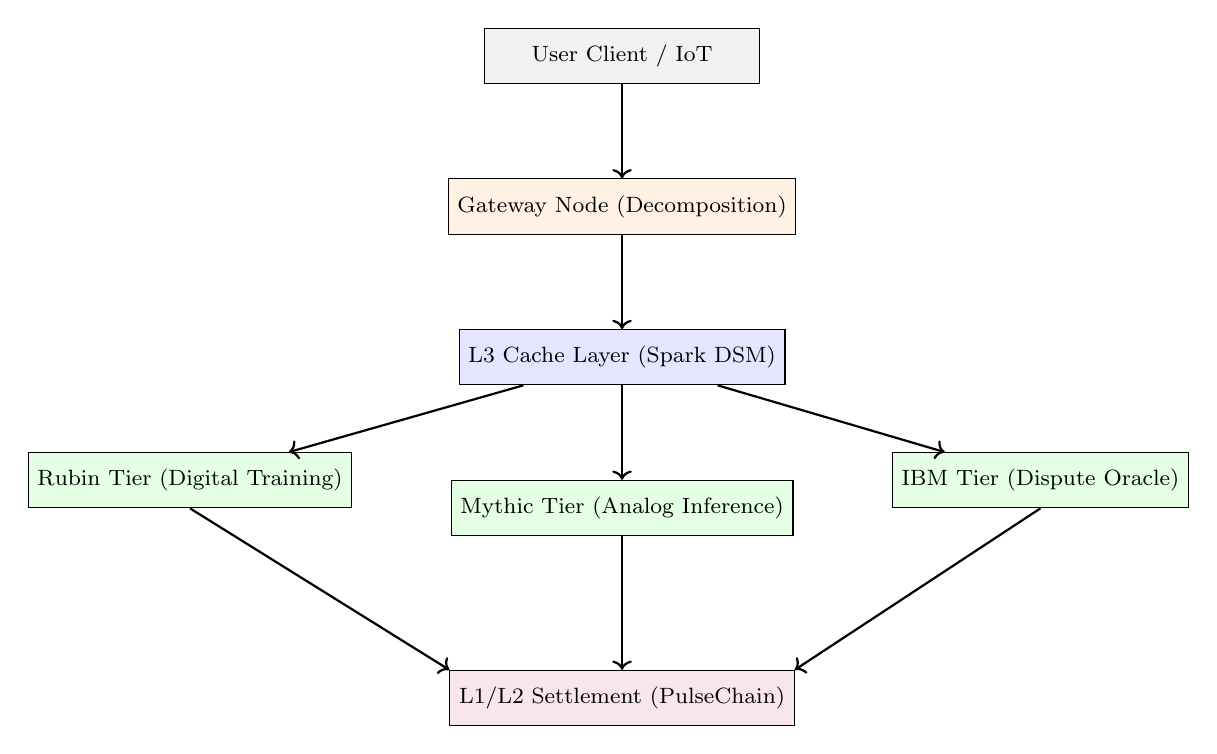
\begin{tikzpicture}[node distance=1.2cm, every node/.style={draw, rectangle, minimum width=3.5cm, minimum height=0.7cm, font=\footnotesize}]
    \node (user) [fill=gray!10] {User Client / IoT};
    \node (gate) [below=of user, fill=orange!10] {Gateway Node (Decomposition)};
    \node (l3) [below=of gate, fill=blue!10] {L3 Cache Layer (Spark DSM)};
    
    % Hardware Tiers
    \node (rubin) [below left=of l3, xshift=-0.5cm, fill=green!10] {Rubin Tier (Digital Training)};
    \node (mythic) [below=of l3, fill=green!10] {Mythic Tier (Analog Inference)};
    \node (quantum) [below right=of l3, xshift=0.5cm, fill=green!10] {IBM Tier (Dispute Oracle)};
    
    \node (settle) [below=of mythic, yshift=-0.5cm, fill=purple!10] {L1/L2 Settlement (PulseChain)};
    
    % Connections
    \draw[->, thick] (user) -- (gate);
    \draw[->, thick] (gate) -- (l3);
    \draw[->, thick] (l3) -- (rubin);
    \draw[->, thick] (l3) -- (mythic);
    \draw[->, thick] (l3) -- (quantum);
    \draw[->, thick] (rubin.south) -- (settle.north west);
    \draw[->, thick] (mythic.south) -- (settle);
    \draw[->, thick] (quantum.south) -- (settle.north east);
\end{tikzpicture}
}
\caption{Layered Stack Architecture: From Edge Submission to Decentralized Settlement.}
\label{fig:stack_arch}
\end{figure}

\section{Risks and Mitigations}
As a decentralized protocol bridging heterogeneous hardware, RAMNET faces several technical risks:
\begin{itemize}
    \item \textbf{Decentralized Latency:} Global scale coordination is limited by WAN physics. \textit{Mitigation:} L3 custom execution environment optimizes micro-coordination, while Gateway Nodes minimize decomposition overhead for edge clients.
    \item \textbf{Analog Precision Drift:} Mythic processors are optimized for efficiency over high-precision floating point operations. \textit{Mitigation:} Analog nodes are prioritized for inference tasks where drift is tolerable, while digital nodes handle high-precision pre-training.
    \item \textbf{FHE Performance Overhead:} Fully Homomorphic Encryption imposes significant compute costs. \textit{Mitigation:} Hybrid execution model where sensitive logic is FHE-wrapped while standard matrix ops utilize Logic-Data Decoupling for native-speed execution.
\end{itemize}

\section{Conclusion}
The RAMNET Protocol represents the inevitable convergence of high-performance digital acceleration, energy-efficient analog signal processing, and post-quantum cryptographic sharding. By formalizing a unified compute mesh that abstracts heterogeneous silicon into a contiguous virtual address space, RAMNET provides the sovereign infrastructure required for the next generation of autonomous intelligence. The integration of next-generation hardware architectures with decentralized resource markets ensures that global compute remains elastic, privacy-preserving, and fundamentally decoupled from the constraints of centralized cloud paradigms.

\bibliographystyle{IEEEtran}
\bibliography{references}

\end{document}
